% A simple compass
% Author: Dario Orescanin

\documentclass{standalone}
\usepackage{tikz}
\usetikzlibrary{calc}
\begin{document}

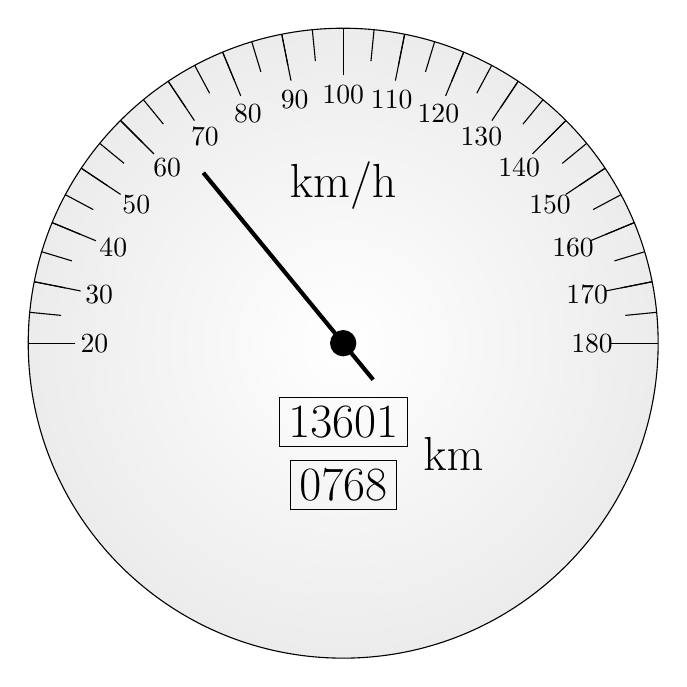
\begin{tikzpicture}[scale=2]
% Define a few constants for easy configuration
\def\radius{2cm}
\def\onedegrad{1.8cm}
\def\fivedegrad{1.75cm}
\def\tendegrad{1.7cm}
\def\labelrad{1.58cm}
\def\nfivetick{33}
\def\ntentick{17}
\pgfmathsetmacro{\stepfivedegree}{180/(\nfivetick-1)}
\pgfmathsetmacro{\steptendegree}{180-180/(\ntentick-1)}
\def\startnum{20}
\def\stepnum{10}
\def\pointerp{65}%指针具体指的数值
\pgfmathsetmacro{\pointerdegree}{180-((\pointerp-\stepnum)/\stepnum -1)*(180/(\ntentick-1))}

% adding a subtle gray tone to add a bit of "personality"
\shade[shading=radial, inner color=white, outer color=gray!15] (0,0) circle (\radius);

\draw (0,0) circle (\radius);

\draw[fill=black] (0,0) circle (0.8mm);
\node[draw, circle, inner sep=.2mm] (a) at (0,0) {};

%指针
\draw[rotate=\pointerdegree,line width=1.5pt] ($(0,0)!1.40cm!(0:1.5cm)$) -- ($(0,0)!-0.3cm!(0:1.5cm)$); 

% main lines
\foreach \x in {0,\stepfivedegree,...,180} \draw (\x:\onedegrad) -- (\x:\radius);


% labels and longer lines at every 10 degrees
\foreach \x [count = \i] in  {180,\steptendegree,...,0}
  { 
  \draw (\x:\tendegrad) -- (\x:\radius);
  \pgfmathsetmacro{\labelnum}{\startnum + (\i-1)*\stepnum}
  \node[] at (\x:\labelrad) {\pgfmathprint{int(\labelnum)}};  
  };


%额外的修改
\node (unit) at (0,1cm) {\LARGE km/h};
\node[draw] (nodea) at (0,-0.5cm) {\LARGE 13601};
\node[draw] (nodeb) at (0,-0.9cm) {\LARGE 0768};
\node[] (nodec) at (0.7cm,-0.7cm) {\LARGE km};

\end{tikzpicture}



\end{document}